\section{Performance Measurements}

Performance measurements were made comparing the transformed code with different
versions of the serial shallow-water code.  The serial versions included two
separate Fortran versions: one using data-parallel notation and the other using
explicit looping constructs.  We also compared with a hand-written OpenCL
implementation that was optimized for local memory usage (no array temporaries).
The accelerated measurements were made using an NVIDIA Tesla C2050 (Fermi) cGPU
with 2.625 GB GDDR5 memory, and 448 processor cores.  The serial measurements
were made using an Intel Xeon X5650 hexacore CPU with 96 GB of RAM running at
2.67 GHz.  The compilers were gfortran and gcc version 4.4.3 with an
optimization level of -O3.

%%TODO All problems were run on a 1280x1280 mesh for 10000 cycles.

%%TODO Timing results were done on a Tesla 1050 class system with an AMD processor (insert info from cat /etc/procinfo and with the DEBUG flag turned on in ezcl.c).

%%The performance comparison is shown in Figure~\ref{fig:cl-performance} for varying array sizes (of the state variables).  The time represents an average of 100 iterations of the outer time-advance loop calling the OpenCL kernel. This tight loop keeps the OpenCL kernel supplied with threads to take advantage of potential latency hiding by the NVIDIA GPU.  Any serial code within this loop would reduce the measured values.

Several timing measurements were made by varying the size of the array state
variables.  The performance measurements are shown in Table~\ref{table:performance}.  An average time was obtained by executing 100 iterations of the outer
time-advance loop that called the OpenCL kernel. This tight loop kept the OpenCL
kernel supplied with threads to take advantage of potential latency hiding by
the NVIDIA GPU.  Any serial code within this loop (not present in this study)
would have reduced the measured values.

\begin{table}
\begin{center}
	\begin{tabular}{|c|c|c|c|}
	\hline Array width & F90 & GPU (16x8) & Speedup \\ \hline\hline
	16   & 0.025 ms & 0.017 ms & 1.5  \\ \hline
	32   & 0.086    & 0.02     & 4.3  \\ \hline
	64   & 0.20     & 0.02     & 10.0 \\ \hline
	128  & 0.76     & 0.036    & 21.1 \\ \hline
	256  & 3.02     & 0.092    & 32.8 \\ \hline
	512  & 12.1     & 0.32     & 37.8 \\ \hline
	1024 & 49.5     & 1.22     & 40.6 \\ \hline
	1280 & 77.7     & 1.89     & 41.1 \\ \hline
	2048 & 199.1    &  4.82    & 41.3 \\ \hline
	4096 & 794.7    & 19.29    & 41.2 \\ \hline
	\end{tabular}
\end{center}
\caption{Performance measurements for the shallow-water code.  All times reported in milliseconds.}
\label{table:performance}
\end{table}

The transformed code achieved very good results.  In all instances, the
performance of the transformed code was within 25\% of the hand-optimized OpenCL
kernel.  Most of the extra performance of the hand-optimized code can be
attributed to the absence of array temporaries and to packing the three state
variables {\tt H, U}, and {\tt V} into a single vector datatype.

While we did not have an OpenMP code for multicore comparisons, the transformed
OpenCL code on the NVIDIA C2050 was up to 40 times faster than the best serial
Fortran code executing on the host CPU.


%\begin{figure}[!t]
%\centering
%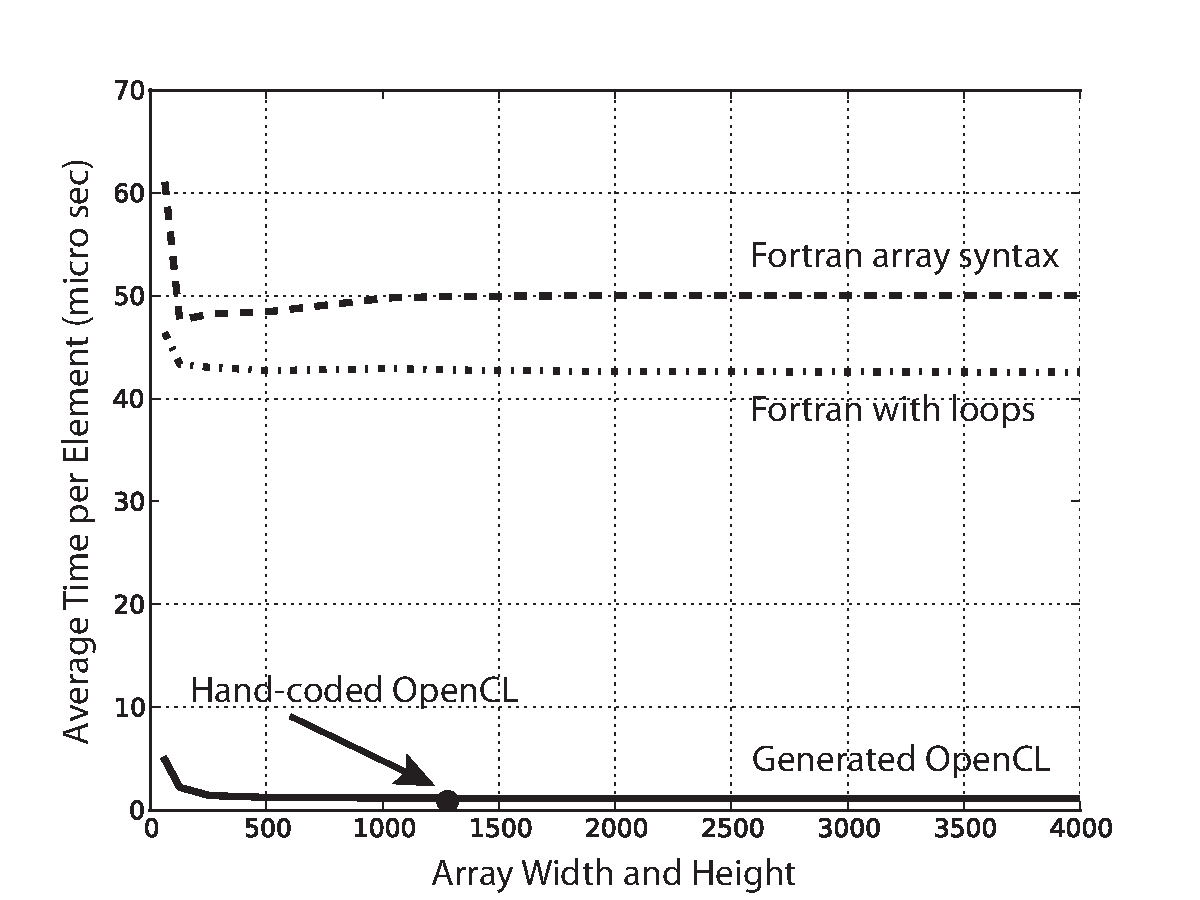
\includegraphics[width=3in]{cl-performance.pdf}
%\caption{Performance comparison for varying array size.}
%\label{fig:cl-performance}
%\end{figure}
